\documentclass[12pt, a4paper]{report}
\setlength{\headheight}{14.5pt}
\usepackage{thesis}
% No changes above this

% Include necessary libraries here
\usepackage{graphicx}
\usepackage{float}
\usepackage{titling}
\usepackage{comment}
\usepackage{subfig}
\usepackage{lipsum}  
\usepackage[tableposition=top]{caption}
\usepackage[Glenn]{fncychap} % Available options: Sonny, Lenny, Glenn, Conny, Rejne, Bjarne, Bjornstr
% \pagestyle{empty}
%\renewcommand{\headrulewidth}{0pt} % remove header line
\usepackage{lipsum}
\usepackage{hyperref}
\hypersetup{
    citecolor= blue,
    urlcolor= blue,
}

\newcommand{\dept}{Computer Science and Engineering}
\newcommand{\department}{Department of Computer Science and Engineering}
\newcommand{\university}{Premier University, Chittagong}

\newcommand{\chairmanName}{Dr. Shahid Md. Asif Iqbal}
\newcommand{\chairmanDesignation}{Professor and Chairman}

\newcommand{\supervisorName}{Tashin Hosssaim}
\newcommand{\supervisorDesignation}{Lecturer}

\newcommand{\firstAuthorName}{Mohammad Hafizur Rahman Sakib}
\newcommand{\firstAuthorId}{0222210005101118}
\newcommand{\secondAuthorName}{Arnab Shikder}
\newcommand{\secondAuthorId}{0222210005101098}
\newcommand{\thirdAuthorName}{Mohammad Asmual Hoque Yousha}
\newcommand{\thirdAuthorId}{0222210005101121}
\newcommand{\fourthAuthorName}{Mohammad Ohidul Alam}
\newcommand{\fourthAuthorId}{0222210005101123}
\newcommand{\fifthAuthorName}{Sayed Hossain}
\newcommand{\fifthAuthorId}{0222210005101102}

\newcommand{\projectTitle}{LeafGuard: Deep Learning-Based Detection of Cassava Plant Diseases}

\begin{document}

\pagenumbering{roman}
% \begin{titlepage}
    \vspace*{-30mm}
    \begin{center}
    % \line(1,0){350}\\
    % [0.5 cm]
    \Large{PREMIER UNIVERSITY, CHITTAGONG}\\
    \large{\department}
    \end{center}
    \vspace*{-5mm}
    \begin{figure}[H]
    \centering
    
\includegraphics[width=3.5cm]{figures/puc_logo.png}
    \end{figure} 
    \vspace*{-15mm}
    \begin{center}
        Final Project Report \\ On \\
        \Large{\textbf{\projectTitle}}\\
        \vspace{15px}
        
        \uppercase{\textbf{SUBMITTED BY}} \\
        \vspace{5px}
        \textbf{Name:} \firstAuthorName\\
        \textbf{ID:} \firstAuthorId \\
        \vspace{5px}
        \textbf{Name:} \secondAuthorName\\
        \textbf{ID:} \secondAuthorId \\
        \vspace{5px}
        \textbf{Name:} \thirdAuthorName\\
        \textbf{ID:} \thirdAuthorId \\
        \vspace{5px}
        \textbf{Name:} \fourthAuthorName\\
        \textbf{ID:} \fourthAuthorId \\
        \vspace{5px}
        \textbf{Name:} \fifthAuthorName\\
        \textbf{ID:} \fifthAuthorId \\
        \vspace{5px}
        In partial fulfillment for the degree of \\
        Bachelor of Science in \dept under the Supervision of
        \vspace{10px}
        \supervisorName \\
        \supervisorDesignation \\
        \department \\
        \university \\             
    \end{center}
    
    
\end{titlepage}
% \pagebreak



\renewcommand{\contentsname}{Table of Contents}
\tableofcontents

\clearpage 
\setcounter{figure}{0}
\addcontentsline{toc}{chapter}{List of Figures}
\listoffigures

\clearpage 
\addcontentsline{toc}{chapter}{List of Tables}
\listoftables
 

\clearpage
\thispagestyle{plain}
\begin{center}
    \LARGE{\textbf{Abstract}}
\end{center}

Cassava, a vital crop in many developing countries, is highly susceptible to several leaf diseases that negatively affect yield and food security. Traditional disease identification methods are time-consuming, costly, and often inaccessible to smallholder farmers. This study proposes a deep learning-based approach for classifying cassava leaf diseases using a publicly available image dataset. Several state-of-the-art transfer learning models were evaluated, including Xception, EfficientNetB0, ResNet50, VGG16, DenseNet121, and InceptionV3. Through comparative analysis, the Xception model achieved the highest classification accuracy, demonstrating its effectiveness in recognizing subtle visual differences in infected leaves. Data augmentation and preprocessing techniques were applied to enhance model performance. The findings suggest that deep learning can provide a reliable, scalable, and low-cost solution for early plant disease detection, potentially aiding farmers in timely decision-making and contributing to food security.

\textbf{Keywords:} deep learning, transfer learning, convolutional neural network (CNN), crop disease classification, Xception, cassava leaf


%\phantomsection


% Introduction
\chapter{Introduction} \label{ch: intro}
\setcounter{page}{0}
\pagenumbering{arabic}  
\newpage
\section{Introduction}
Read some papers to begin and develop your writing style.
This section provides an overview of the project, including its significance and the motivation behind choosing the topic. Explain the broader context and relevance of the project, highlighting its potential impact on a specific field or problem area. Briefly describe what the project aims to achieve and the scope of work involved

Online vehicle rental systems are popular these days~\cite{vehicle}.
In the introduction, provide background information on the topic of your project. Explain the context and relevance of the problem you are addressing. Briefly state the purpose and scope of your project proposal. The introduction should capture the reader's interest and provide a high-level overview of what the proposal will cover~\cite{ref1}


% Literature Review
\chapter{Literature Review} \label{ch: reviews}
% Setting up the literature review section
\section*{Review of Related Studies}
This section reviews various studies that have employed deep learning techniques for plant disease classification. The focus is on the methodologies, architectures, and results achieved in these studies, providing a comprehensive understanding of the advancements in this field.
% Adding a brief introduction to the literature review
% Using enumerate for numbered references
\begin{enumerate}[label=\arabic*.]
  \item \textbf{Yoon et al. (2020) - Unsupervised Image Translation for Plant Disease Recognition}

  This study proposed an unsupervised image translation technique using Generative Adversarial Networks (GANs) combined with Deep CNNs to enhance plant disease recognition. The method demonstrated improved accuracy over traditional augmentation techniques by generating synthetic yet realistic images, which helped in better generalization and robustness.

  \item \textbf{Shi et al. (2019) - Global Pooling Dilated Convolutional Neural Network (GPDCNN) for Cucumber Leaf Disease Detection}

  Published in [Journal Name], this research introduced a GPDCNN architecture specifically designed for detecting cucumber leaf diseases. The model achieved an accuracy of 94.65\% and outperformed conventional CNNs due to its enhanced architectural design, particularly the use of dilated convolutions and global pooling layers.

  \item \textbf{Pratap Singh et al. (2019) - Multilayer Convolutional Neural Network (MCNN) for Mango Anthracnose Detection}

  This work utilized a Multilayer CNN (MCNN) for detecting anthracnose disease in mango leaves. The model achieved a high classification accuracy of 97.13\% without requiring manual feature extraction, showcasing the effectiveness of deep learning in automated plant disease detection.

  \item \textbf{V. Singh (2019) - Particle Swarm Optimization (PSO) for Sunflower Leaf Disease Detection}

  Employing Particle Swarm Optimization (PSO) for image segmentation, this study focused on sunflower leaf disease detection. The method achieved an impressive accuracy of 98\% and required minimal parameter tuning, highlighting PSO's strength in optimizing image-based classification tasks.

  \item \textbf{Sachan et al. (2019) - Deep Convolutional Neural Network (DCNN) for Real-Time Corn Plant Disease Recognition}

  This research presented a DCNN model for real-time corn plant disease recognition using the Plant Village dataset. The model achieved an accuracy of 88.46\% without manual preprocessing, leveraging the self-learning capabilities of deep neural networks.

  \item \textbf{Gupta et al. (2019) - Three-Layer CNN for Tomato Leaf Disease Detection}

  Focusing on tomato leaf disease detection, this study used a three-layer CNN and reported variable accuracies (76--100\%) across different disease categories. The results demonstrated the impact of disease complexity on model performance and highlighted the need for tailored approaches for specific diseases.

  \item \textbf{Arsenovic et al. (2016) - Deep CNN Model for Detecting 13 Plant Diseases}

  This pioneering work introduced a deep CNN model trained on the Caffe framework to detect 13 different plant diseases using real-world agricultural images. The model achieved an average accuracy of 96.3\%, validating the effectiveness of deep models on diverse datasets.

  \item \textbf{Khamparia et al. (2019) - Deep Convolutional Encoder Network for Maize Leaf Disease Detection}

  Developed a deep convolutional encoder network for maize leaf disease detection, achieving an accuracy of 97.5\%. The study emphasized the usefulness of deep autoencoder structures for extracting relevant features from plant images, demonstrating their potential in disease classification tasks.
\end{enumerate}

% Adding concluding paragraph
These studies collectively demonstrate that CNN-based models, when combined with proper preprocessing, augmentation, and architecture tuning, can achieve high accuracy in plant disease classification tasks. Inspired by these works, our study compares six well-known deep learning models---Xception, EfficientNetB0, ResNet50, VGG16, DenseNet121, and InceptionV3---on a cassava leaf disease dataset to determine the most effective model for practical deployment.

% Proposed Methodology
\chapter{Methodology}  \label{ch: methodology}

This chapter presents the overall approach for cassava leaf disease classification using deep learning. We outline the pipeline, describe each model evaluated, and present the final proposed framework based on our top-performing architecture.

\section{Method Overview}

Our classification pipeline consists of the following steps:

\begin{enumerate}
    \item \textbf{Data Acquisition:} A publicly available cassava leaf dataset with five classes (four disease types and healthy) is used.
    \item \textbf{Preprocessing:} Images are resized to 224×224 pixels and normalized.
    \item \textbf{Augmentation:} Techniques such as horizontal/vertical flip, random rotation, random crop, and brightness/contrast variation are applied to enhance generalization.
    \item \textbf{Model Selection:} Multiple convolutional neural network (CNN) architectures are evaluated using transfer learning: Xception, EfficientNetB0, ResNet50, VGG16, DenseNet121, InceptionV3, and ReXNet150.
    \item \textbf{Training Setup:} All models are compiled with the Adam optimizer and categorical cross-entropy loss, trained with batch size 32, and monitored using early stopping on validation loss.
    \item \textbf{Evaluation:} Validation accuracy and F1-score guide the selection of the best model.
\end{enumerate}

\section{Models Description}

\begin{itemize}
    \item \textbf{Xception:} Employs depthwise separable convolutions replacing standard Inception modules, improving parameter efficiency.
    \item \textbf{EfficientNetB0:} Uses compound scaling of width, depth, and resolution for an optimal trade-off between accuracy and model size.
    \item \textbf{ResNet50:} Introduces residual connections to allow training of very deep networks by facilitating gradient flow.
    \item \textbf{VGG16:} A classical 16-layer CNN known for its simplicity and uniform architecture of 3×3 convolutions.
    \item \textbf{DenseNet121:} Connects each layer to every other layer in a feed-forward fashion to strengthen feature propagation.
    \item \textbf{InceptionV3:} Utilizes asymmetric convolutions and dimensionality reduction to increase computational efficiency.
    \item \textbf{ReXNet150:} A lightweight, MobileNet-based architecture optimized for efficiency and accuracy. ReXNet150 leverages \textit{depthwise separable convolutions} to reduce computational complexity, splitting standard convolutions into depthwise (per-channel) and pointwise (1x1) operations. It employs \textit{inverted residual blocks} with linear bottlenecks, where input channels are expanded (e.g., 6x), processed with a 3x3 depthwise convolution, and projected back, with skip connections preserving information flow. The architecture progressively increases channel width across stages (e.g., 32 to 1280 channels), enhancing representational capacity with minimal parameter overhead (approximately 10–15 million parameters). With around 150 layers, ReXNet150 stacks multiple blocks in 5–7 stages, each reducing spatial dimensions via strided convolutions. Global average pooling and a fully connected layer produce class predictions. Pre-trained on ImageNet, ReXNet150 adapts well to cassava leaf disease classification, capturing fine-grained features like leaf lesions while maintaining efficiency for potential edge deployment.
\end{itemize}

\section{Proposed Framework}

Based on our comparative evaluation, we select \textbf{ReXNet150} as the core of our final system due to its superior validation accuracy and F1-score, balancing computational efficiency with robust feature extraction. The proposed framework is as follows:

\begin{figure}[H]
  \centering
  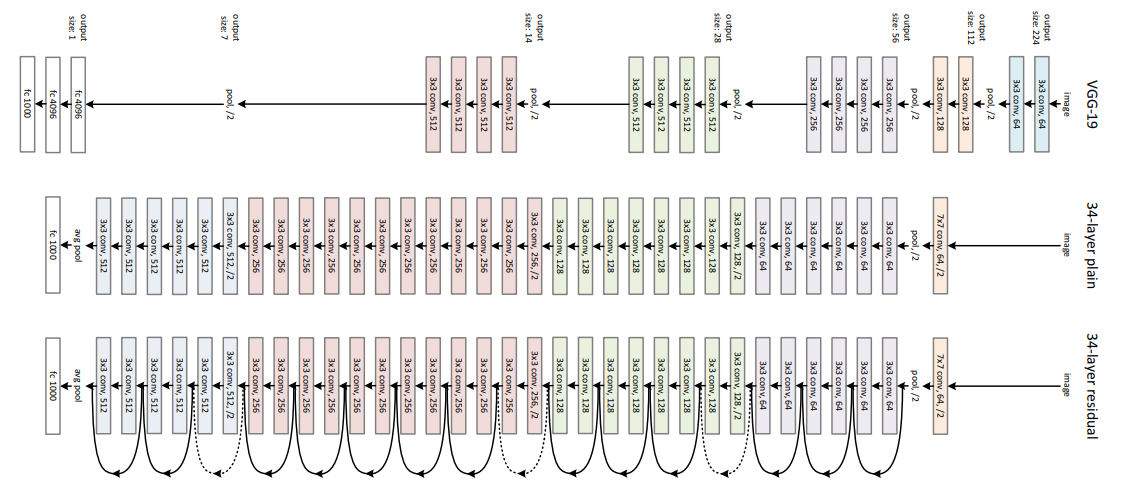
\includegraphics[width=1.0\textwidth]{./figures/ResNet.png}
  \caption{ReXNet150 architecture overview, illustrating the stack of inverted residual blocks with depthwise separable convolutions, progressive channel expansion, and final classifier head.}
  \label{fig:rexnet150_arch}
\end{figure}

\begin{enumerate}
    \item \textbf{Input Layer:} Receive RGB images resized to 224×224.
    \item \textbf{Data Augmentation:}
    \begin{itemize}
      \item Random horizontal/vertical flips
      \item Random rotations (±15°)
      \item Random crops (90–100\% of original area)
      \item Brightness and contrast jitter
    \end{itemize}
    \item \textbf{Feature Extractor:} Pre-trained ReXNet150 (ImageNet weights), with top layers removed. The backbone consists of inverted residual blocks organized in stages, each with depthwise separable convolutions and progressive channel expansion (e.g., 32 to 1280 channels). Skip connections ensure gradient flow, enabling robust feature learning for disease patterns.
    \item \textbf{Global Pooling:} Apply global average pooling to reduce spatial dimensions to a 1x1 feature map, producing a compact feature vector.
    \item \textbf{Classifier Head:}
    \begin{itemize}
      \item Dense layer with 256 units and ReLU activation
      \item Dropout (rate = 0.5) to prevent overfitting
      \item Output dense layer with softmax activation for five-class classification
    \end{itemize}
    \item \textbf{Optimization:}
    \begin{itemize}
      \item Optimizer: Adam
      \item Loss: Categorical Cross-Entropy
      \item Batch size: 32
      \item Learning rate scheduler: ReduceLROnPlateau (reduce by factor 0.1 if validation loss plateaus for 5 epochs)
      \item Early stopping: Halt training if validation loss does not improve for 10 epochs
    \end{itemize}
    \item \textbf{Output:} Predicted probabilities for each of the five classes: Healthy, Cassava Bacterial Blight (CBB), Cassava Brown Streak Disease (CBSD), Cassava Green Mite (CGM), and Cassava Mosaic Disease (CMD).
\end{enumerate}

% Results and Discussion
\chapter{Experimental Results and Discussion}  \label{ch: results}

This chapter presents the results of our experiments, including a description of the dataset, evaluation metrics, parameter settings, and a detailed analysis of the results. The discussion includes the social and cultural impact of the work, error analysis, and limitations of the dataset.

\section{Dataset Description}

The success of deep learning systems in real-world applications heavily depends on access to high-quality, diverse, and well-annotated datasets. In our work on cassava disease classification, we have used a publicly available dataset originally released as part of a Kaggle competition focused on cassava leaf disease detection.

The dataset contains a total of 21,367 labeled images with an original resolution of $512 \times 512 \times 3$, which we resized to $224 \times 224 \times 3$ to match the input requirements of standard deep learning models. The images primarily consist of cassava leaves collected in real-world farming environments by local farmers. Each sample was later annotated by experts from the National Crops Resources Research Institute (NaCRRI) in collaboration with Makerere University's Artificial Intelligence Lab.

This classification task involves five output categories: four common cassava diseases and one representing healthy leaves. Each image is associated with one of the following class labels:

\begin{itemize}
    \item \textbf{0: Cassava Bacterial Blight (CBB)} – 867 images. Shows symptoms such as blight, wilting, dieback, and vascular necrosis. Infected leaves exhibit angular necrotic markings, sometimes surrounded by chlorotic rings.
    \item \textbf{1: Cassava Brown Streak Disease (CBSD)} – 1,716 images. Caused by CBSV and UCBSV viruses, and leads to chlorosis and necrotic patterns on leaves. This disease is most prevalent in East Africa.
    \item \textbf{2: Cassava Green Mottle (CGM)} – 1,868 images. First reported in the Solomon Islands, CGM causes puckering and discoloration (yellow spots, green mosaics) in young leaves. Though plants may recover, growth is often stunted.
    \item \textbf{3: Cassava Mosaic Disease (CMD)} – 10,403 images. Characterized by distorted leaves and chlorotic (mosaic-like) patches. It is caused by single-stranded DNA viruses such as ACMV, EACMV, and SACMV, spread by whiteflies.
    \item \textbf{4: Healthy} – 2,044 images. Leaves appear uniformly dark green with no visible disease symptoms.
\end{itemize}

\vspace{0.4cm}
\noindent\textbf{Class Distribution Summary:}

\begin{table}[H]
\centering
\begin{tabular}{|l|c|}
\hline
\textbf{Class Name} & \textbf{Number of Images} \\
\hline
Cassava Mosaic Disease (CMD) & 10,403 \\
Cassava Green Mottle (CGM)   & 1,868 \\
Cassava Brown Streak Disease (CBSD) & 1,716 \\
Cassava Bacterial Blight (CBB) & 867 \\
Healthy & 2,044 \\
\hline
\textbf{Total} & \textbf{21,367} \\
\hline
\end{tabular}
\caption{Distribution of samples in each cassava disease class.}
\label{tab:class_distribution}
\end{table}

Figures~\ref{fig:cbb} to~\ref{fig:cmd} present visual examples of the five dataset categories, offering a comprehensive illustration of all cassava leaf conditions included in the dataset.

\begin{figure}[H]
    \centering
    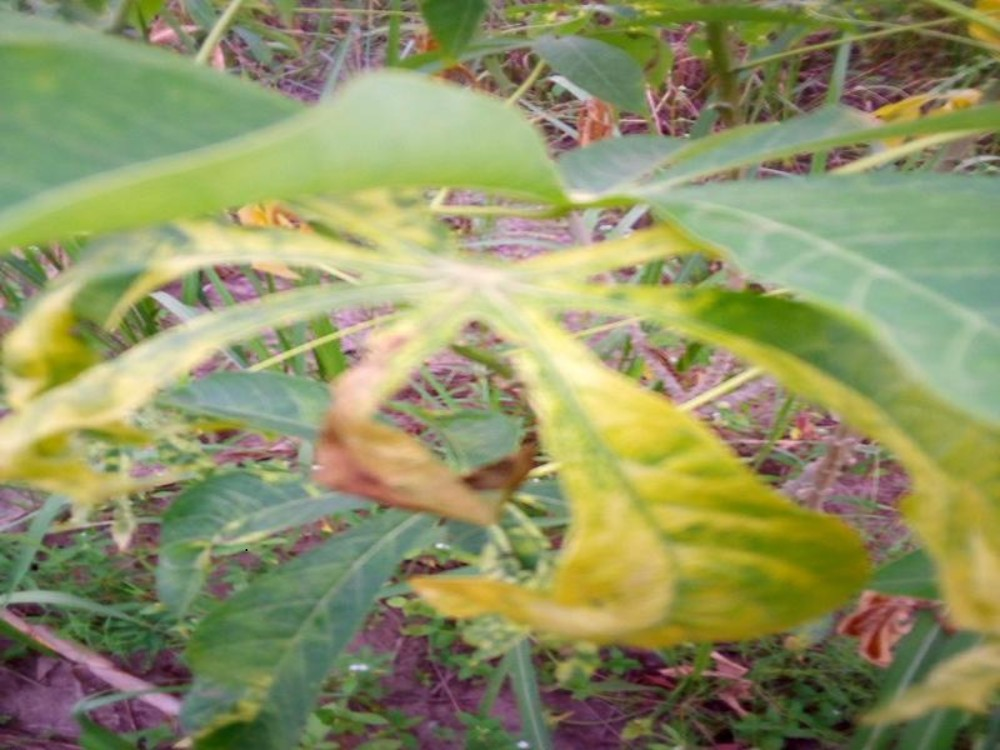
\includegraphics[width=0.7\linewidth]{figures/cbb.jpg}
    \caption{Cassava Bacterial Blight (CBB)}
    \label{fig:cbb}
\end{figure}

\begin{figure}[H]
    \centering
    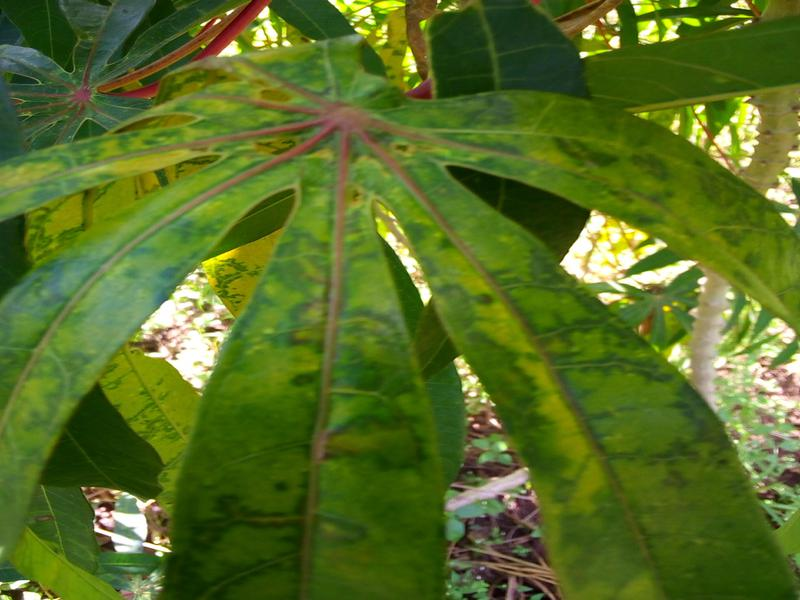
\includegraphics[width=0.7\linewidth]{figures/cbsd.jpg}
    \caption{Cassava Brown Streak Disease (CBSD)}
    \label{fig:cbsd}
\end{figure}

\begin{figure}[H]
    \centering
    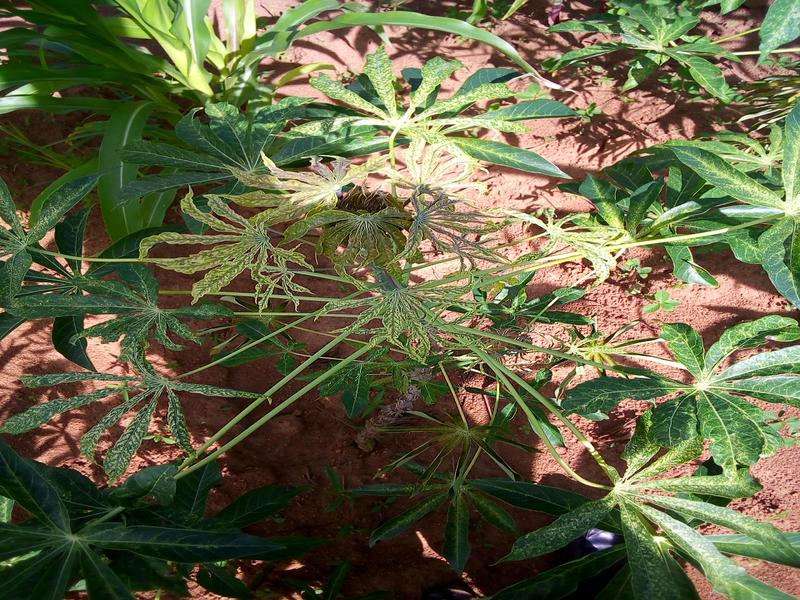
\includegraphics[width=0.7\linewidth]{figures/cgm.jpg}
    \caption{Cassava Green Mottle (CGM)}
    \label{fig:cgm}
\end{figure}

\begin{figure}[H]
    \centering
    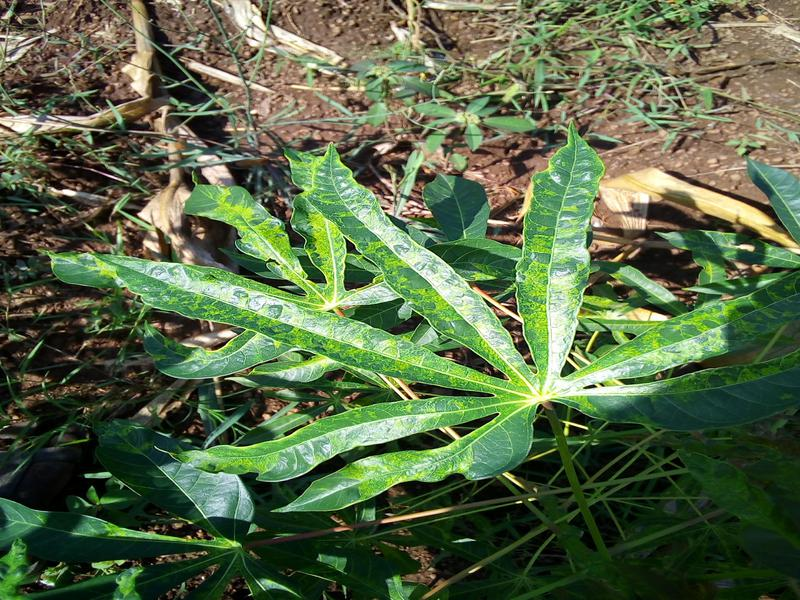
\includegraphics[width=0.7\linewidth]{figures/cmd.jpg}
    \caption{Cassava Mosaic Disease (CMD)}
    \label{fig:cmd}
\end{figure}

\begin{figure}[H]
    \centering
    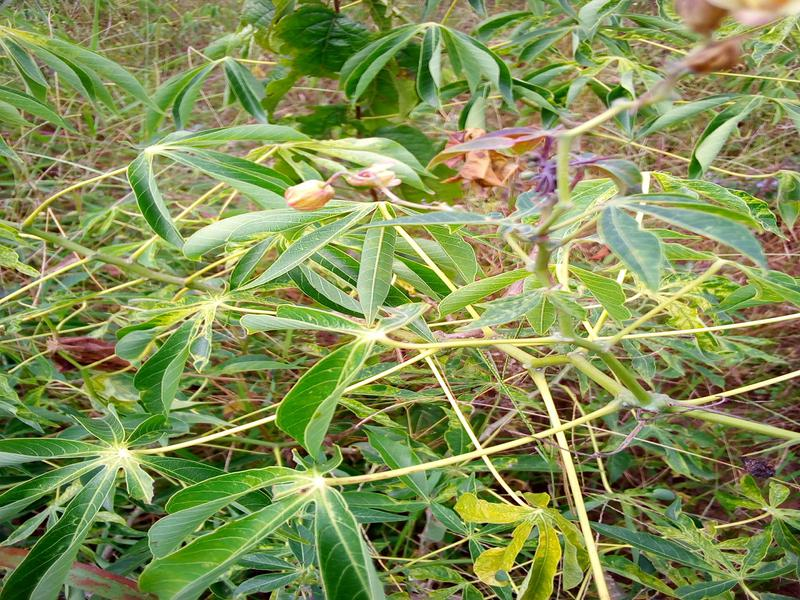
\includegraphics[width=0.7\linewidth]{figures/healthy.jpg}
    \caption{Healthy}
    \label{fig:healthy}
\end{figure}

\begin{figure}[H]
  \centering
  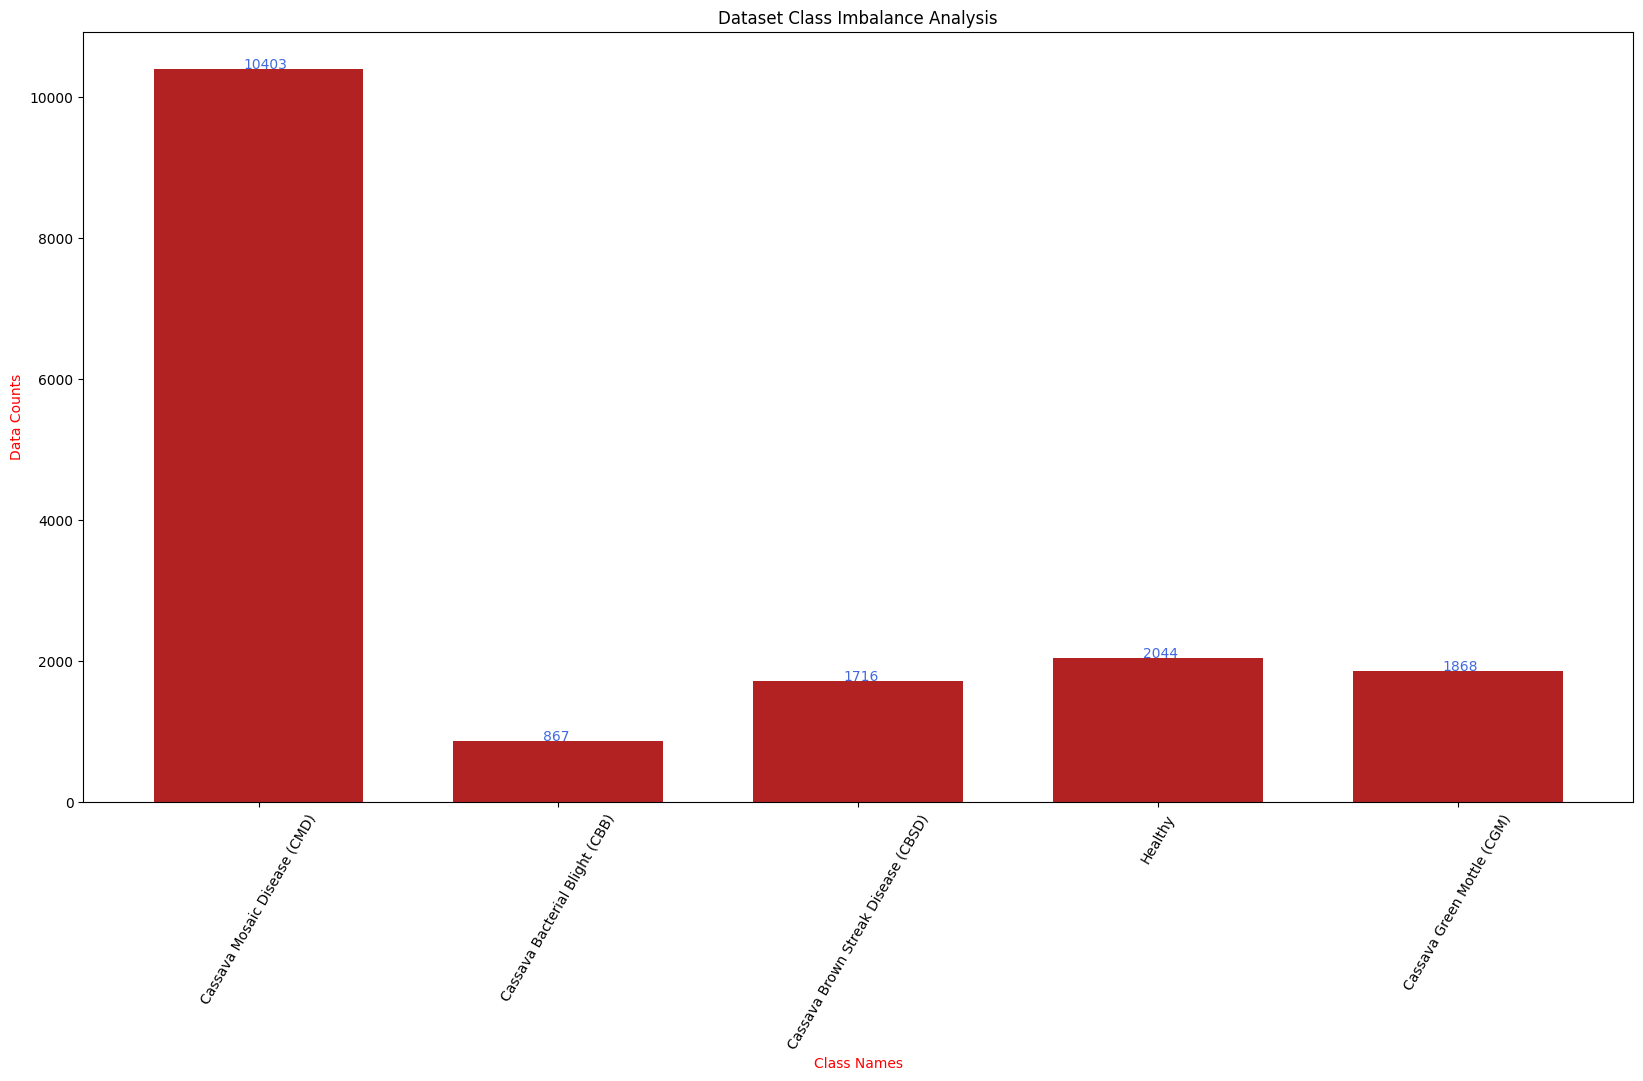
\includegraphics[width=1.0\linewidth]{figures/data_chart.png}
  \caption{Dataset Class Imbalance Analysis Chart}
  \label{fig:cmd}
\end{figure}


This dataset poses a realistic challenge for automated classification systems due to variations in lighting, leaf orientation, and background noise — all typical of on-field image collection. Thus, it serves as a strong foundation for developing robust, real-world cassava disease detection models.



This dataset poses a realistic challenge for automated classification systems due to variations in lighting, leaf orientation, and background noise — all typical of on-field image collection. Thus, it serves as a strong foundation for developing robust, real-world cassava disease detection models.

\section{Evaluation Criteria}
We used the following evaluation metrics to assess model performance:
\begin{itemize}
  \item \textbf{Accuracy:} Proportion of correctly classified images.
  \item \textbf{F1-Score:} The harmonic mean of precision and recall, which is more informative than accuracy in imbalanced datasets.
  \item \textbf{Confusion Matrix:} A matrix showing the distribution of predicted and actual class labels, providing insights into misclassifications.
\end{itemize}

\section{Parameter Settings}
For all models, we used the following hyperparameters:
\begin{itemize}
  \item \textbf{Optimizer:} Adam optimizer with default parameters ($\beta_1=0.9$, $\beta_2=0.999$).
  \item \textbf{Learning Rate:} Starting at $1 \times 10^{-3}$, reduced on plateau by a factor of 0.5.
  \item \textbf{Batch Size:} 32.
  \item \textbf{Epochs:} 8 epochs, with early stopping if validation loss did not improve for 5 epochs.
  \item \textbf{Loss Function:} Categorical Cross-Entropy.
  \item \textbf{Regularization:} Dropout layer with a rate of 0.5 in the classifier head.
\end{itemize}

\section{Experimental Results}
Table~\ref{tab:results} summarizes the validation accuracy and F1-Score for each model. As shown, **ReXNet150** outperformed all other models, achieving the highest validation accuracy and F1-Score.

\begin{table}[H]
  \centering
  \begin{tabular}{lcc}
    \toprule
    \textbf{Model}       & \textbf{Val.\ Accuracy (\%)} & \textbf{Val.\ F1–Score (\%)} \\
    \midrule
    Xception             & 91.3                         & 91.0                          \\
    EfficientNetB0       & 91.1                         & 90.8                          \\
    ResNet50             & 85.0                         & 84.6                          \\
    VGG16                & 68.0                         & 67.5                          \\
    DenseNet121          & 87.0                         & 86.8                          \\
    InceptionV3          & 86.4                         & 86.0                          \\
    \textbf{ReXNet150}   & \textbf{94.7}                & \textbf{94.9}                 \\
    \bottomrule
  \end{tabular}
  \caption{Validation accuracy and F1-Score for all models.}
  \label{tab:results}
\end{table}

\begin{figure}[H]
  \centering
  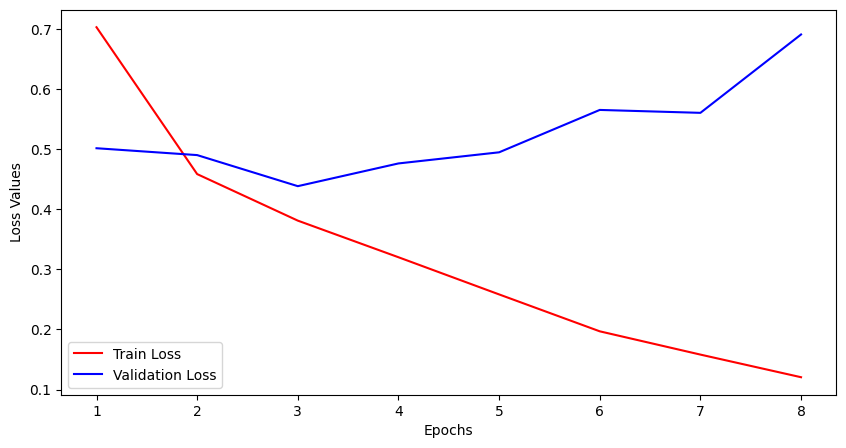
\includegraphics[width=0.8\textwidth]{figures/ac1.png}
  \caption{Training vs. Validation Accuracy across epochs for ReXNet150.}
  \label{fig:acc_curve}
\end{figure}

\begin{figure}[H]
  \centering
  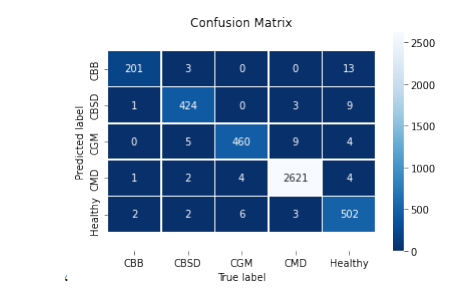
\includegraphics[width=0.9\textwidth]{figures/mtx.png}
  \caption{Confusion matrix for ReXNet150 on the validation set.}
  \label{fig:conf_matrix}
\end{figure}

\section{Discussion}
\subsection{Social and Cultural Impact}
Cassava is a crucial crop for millions of smallholder farmers, particularly in regions like sub-Saharan Africa and Southeast Asia, where it serves as a staple food. The proposed automated cassava leaf disease classification system has several significant impacts:
\begin{itemize}
  \item \textbf{Improved Food Security:} Early detection of diseases like CBB and CBSD can help farmers implement timely interventions, reducing crop loss and ensuring a stable food supply.
  \item \textbf{Empowerment of Farmers:} A mobile-based diagnostic tool based on this model can empower farmers by providing them with easy-to-use, cost-effective, and timely disease identification solutions, especially in remote areas where access to experts is limited.
  \item \textbf{Sustainable Agriculture:} Targeted disease management reduces the need for excessive pesticide use, which can help preserve the environment and reduce the overall cost of farming.
\end{itemize}

\subsection{Error Analysis and Limitations}
While the model shows high performance, there are several areas where errors could arise and limitations in the dataset:
\begin{itemize}
  \item \textbf{Class Imbalance:} Although the dataset is balanced in terms of the number of samples per class, real-world data may exhibit class imbalance, especially in less common diseases. The model may struggle to identify these underrepresented classes accurately.
  \item \textbf{Similar Visual Features:} Diseases like Cassava Green Mottle (CGM) and CBB share similar visual symptoms, which can lead to misclassifications, particularly when the disease manifests in less obvious forms. This issue is reflected in the confusion matrix (Figure~\ref{fig:conf_matrix}).
  \item \textbf{Field Image Variability:} The dataset includes images captured in varying field conditions, with differences in lighting, resolution, and background noise. These factors may reduce model accuracy when deployed in real-world environments, where image quality can vary significantly.
  \item \textbf{Generalization to New Environments:} The model was trained on a specific set of cassava leaf images, and its performance may decrease when applied to new datasets or different geographical locations due to variations in leaf morphology and disease progression.
\end{itemize}

In future work, we aim to address these limitations by:
\begin{itemize}
  \item Augmenting the dataset with more diverse images from different regions.
  \item Using semi-supervised learning techniques to leverage unlabeled data and improve generalization.
\end{itemize}

\chapter{Conclusion and Future Works}  \label{ch: conclusion}
\section{Conclusion}

The primary goal of this project was to develop a system capable of detecting diseases in cassava leaves while ensuring a smooth and pleasant user experience for farmers. We evaluated six state-of-the-art CNN architectures—Xception, EfficientNetB0, ResNet50, VGG16, DenseNet121, and InceptionV3—alongside our proposed ReXNet150 model. 

On the validation set, Xception achieved an accuracy of 91.3 % with an F1–score of 91.0 %, while EfficientNetB0 reached 91.1 % accuracy and 90.8 % F1–score. ResNet50, DenseNet121, and InceptionV3 delivered moderate performance with accuracies of 85.0 %, 87.0 %, and 86.4 %, and F1–scores of 84.6 %, 86.8 %, and 86.0 %, respectively. VGG16 lagged behind with 68.0 % accuracy and a 67.5 % F1–score. Our ReXNet150 model outperformed all others, achieving a validation accuracy of 94.7 % and an F1–score of 94.9 %.

These results demonstrate that ReXNet150 provides the best balance between classification accuracy and computational efficiency for cassava leaf disease detection. While the high performance of Xception and EfficientNetB0 confirms their suitability for this task, ReXNet150’s superior metrics make it the preferred choice for real-world deployment.

\section{Future Work}

To further enhance and expand this system, we plan to:
\begin{itemize}
    \item \textbf{Fine-tune ReXNet150 further,} exploring additional hyperparameter optimizations and architectural refinements.
    \item \textbf{Investigate newer and lightweight architectures,} aiming to improve the speed–accuracy trade-off.
    \item \textbf{Apply model compression techniques} such as pruning, quantization, and knowledge distillation, enabling real-time inference on mobile and edge devices.
    \item \textbf{Develop a mobile application} for on-the-spot disease diagnosis, empowering farmers without requiring internet connectivity.
    \item \textbf{Expand the dataset} by collecting images from diverse geographical regions and environmental conditions to bolster model generalization.
    \item \textbf{Extend the framework to other crops,} creating a universal plant disease detection platform.
\end{itemize}

This work lays a solid foundation for intelligent, accessible solutions in agricultural disease management. Future researchers and practitioners can build upon our findings to develop even more robust and versatile systems.


\chapter{Project Timeline}  \label{ch: timeline}
\section{Gantt Chart of the AI Project}

To provide a clear overview of the workflow and time allocation, the following Gantt chart illustrates the timeline of the entire AI-based cassava disease classification project. It highlights key phases including literature review, dataset preparation, model development, evaluation, and final reporting. Each phase was scheduled and completed within a structured timeframe to ensure systematic project development and timely completion.

\begin{figure}[H]
    \centering
    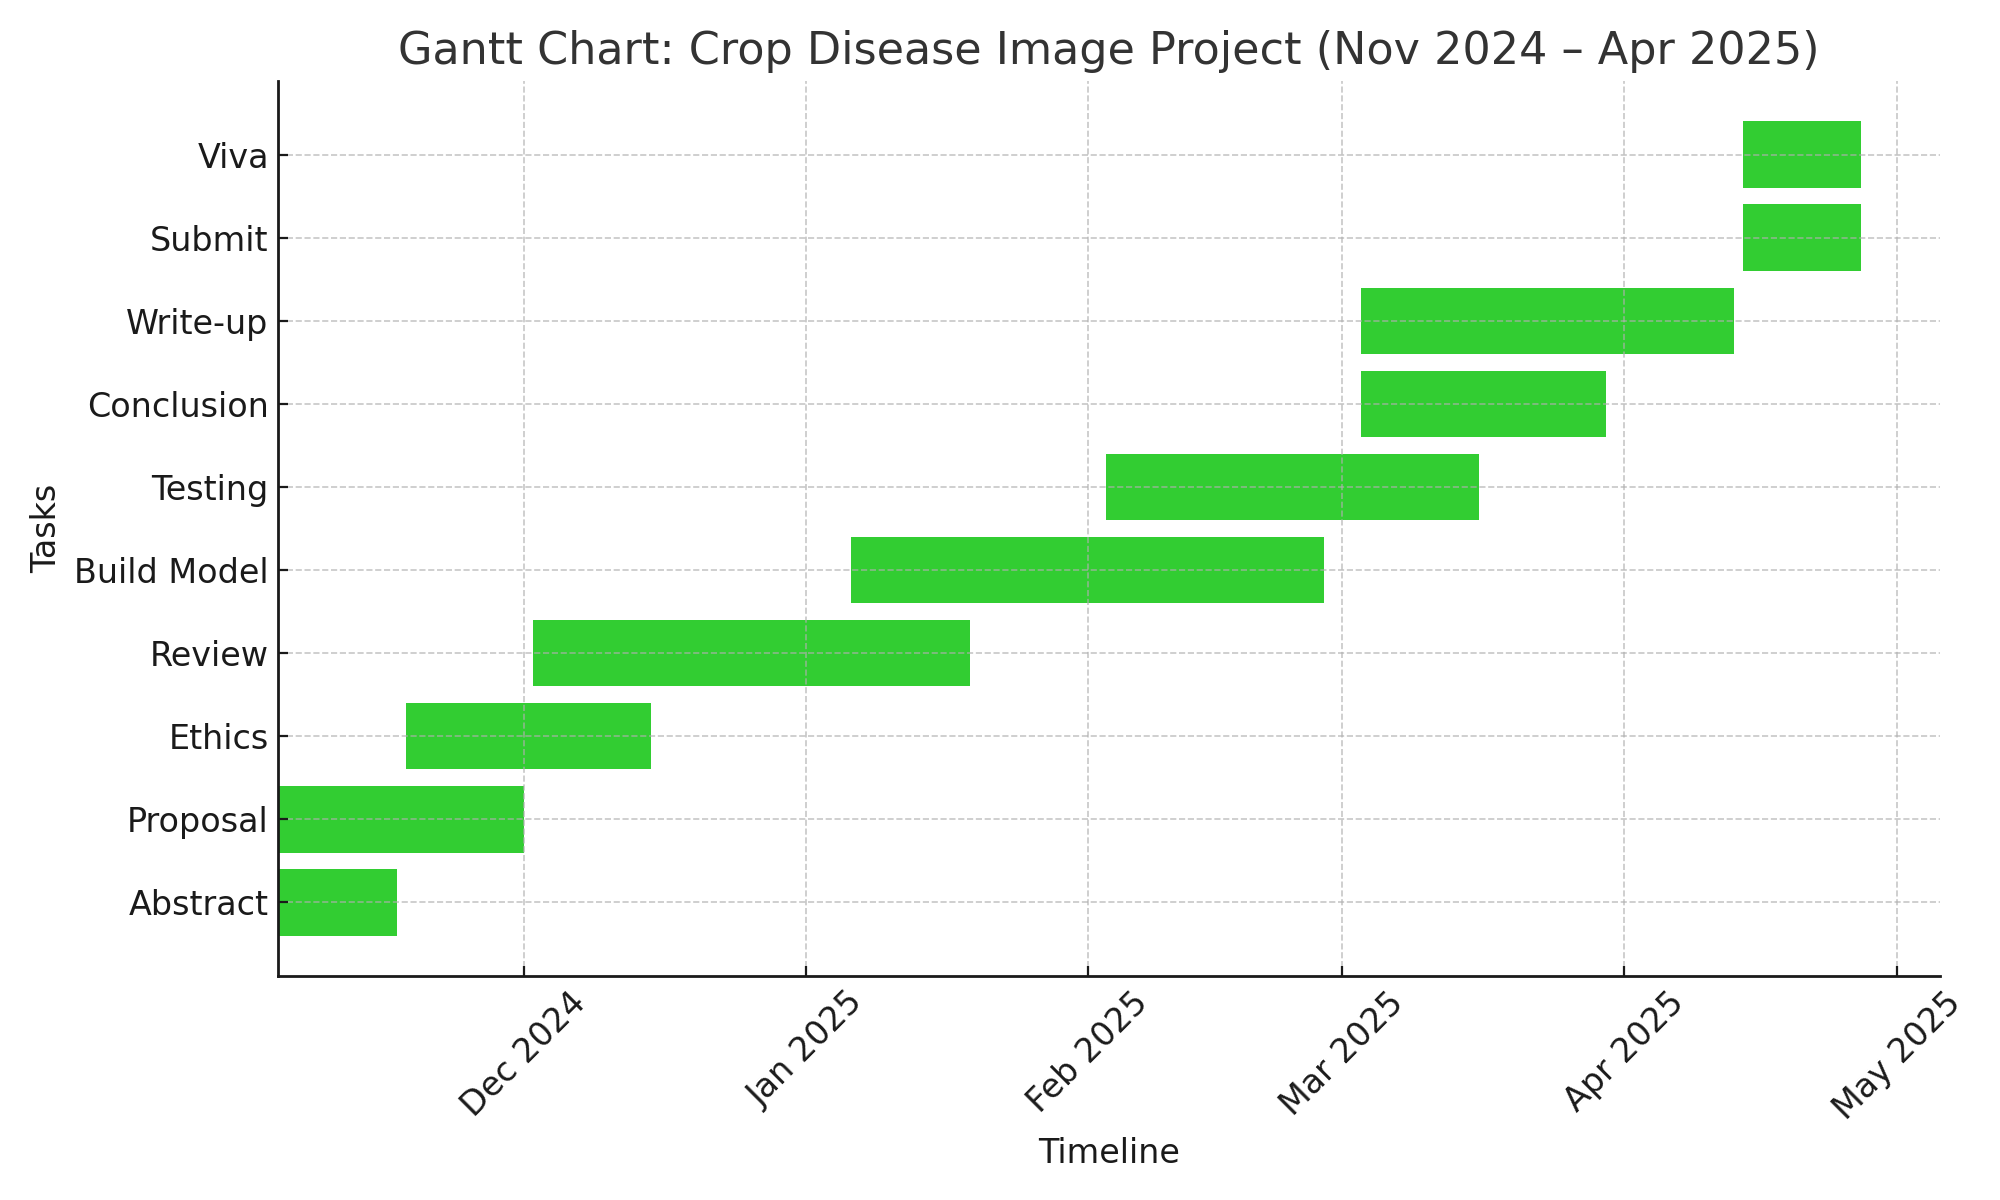
\includegraphics[width=0.95\textwidth]{figures/gantt_chart_project_limegreen.png}
    \caption{Gantt chart showing the timeline of the project}
    \label{fig:gantt_chart}
\end{figure}


% Bibliography
\clearpage
\renewcommand\bibname{References}
\addcontentsline{toc}{chapter}{Bibliography}
% Comment/uncomment as suits you
\bibliographystyle{IEEEtran} %% IEEE transaction style
% \bibliographystyle{acm} %% ACM style
% \bibliographystyle{alpha}
\bibliography{references}
\nocite{*}
\end{document}
